\biohead{Catherine Aldridge}{Date unknown.\cite{CaltherineAldridgePortrait}}

Catherine Aldridge was born on 7 Dec 1847, in Hornsey \cite{JHMtree, 1881censusKingston} to Napoleon Aldridge (\p{Napoleon_Aldridge}) and Mary Ann Chymist (\p{Mary_Ann_Chymist}).  She had seven siblings, who were: Edward Henry Aldridge (1832--1899), Napoleon Alfred Aldridge (1836--1905), Leah North Aldridge (1837--1912), Virginia Elizabeth Aldridge (1839--1912), William Aldridge (1843--?), Alice Judith Aldridge (1845--?) and Alfred Frank Aldridge (1846--?).

She married John Hill Munday (aged 32) on 8 April 1880\cite{JHM-CA-marriage} at Benhilton Church in Sutton (near Croydon, Surrey).\cite{JHM-CA-marriage, JHM-CA-marriage-announcement}

In April 1881 she was living at 8 Shalston Villas, Ewell Road.\cite{1881censusKingston}

In April 1891, Catherine and John Hill were living at the Mendips and they had four servants, with the gardener and coachman living next door at Mendip Stables.\cite{1891census} In 1901, they were still there and only Nora and Margery were at home (the others were away at school) with the servants consisting of Cook, 2 parlourmaids, housemaid, domestic, kitchenmaid, and coachman.\cite{1901censusMendips}

By 1911, the family had moved to Cedar Lodge at 21 St Johns Road in Putney Hill (Catherine was 63); all five children were at home, and they had three servants: Cook, housemaid and parlourmaid.\cite{1911censusWandsworth}

She died in June 1922 in Birkenhead.\cite{FreeBMD-CA} After her death her children sent the following card: ``The Son and Daughters of the late Mrs. J. H. Munday return thanks for all the kindness and sympathy shown to them in their bereavement. (26 Devonshire Road, Claughton, Birkenhead.)''\cite{CA-bereavement-card}

\begin{figure}
	\centering
	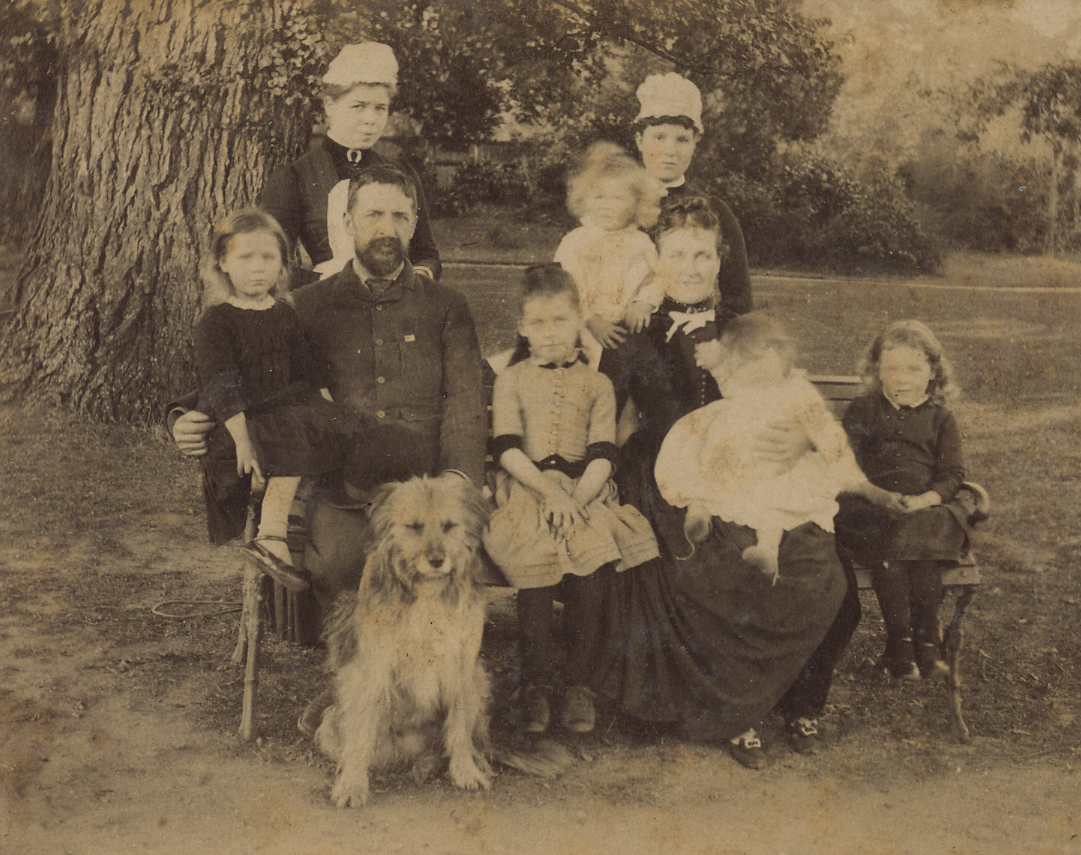
\includegraphics{photos/JH_Munday_and_family_1888.png}
	\caption{The Munday family, Sunday 21 October 1888.}
\end{figure}

\begin{figure}
	\centering
	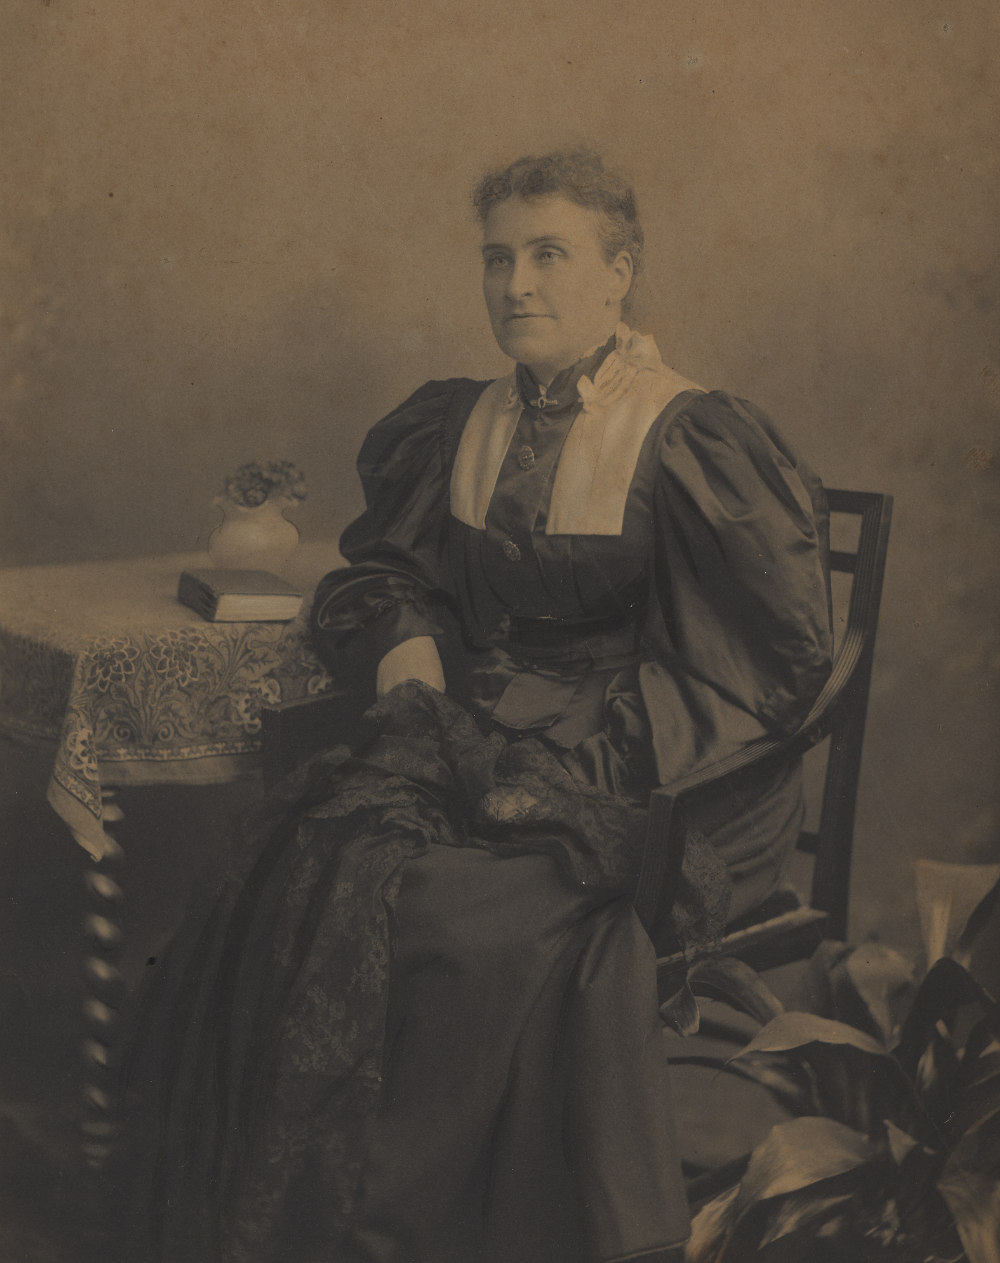
\includegraphics{photos/Catherine_Aldridge_1895-09-28.png}
	\caption{28 September 1895.}
\end{figure}

\begin{figure}
	\centering
	\label{MundayFamilyPhoto}
	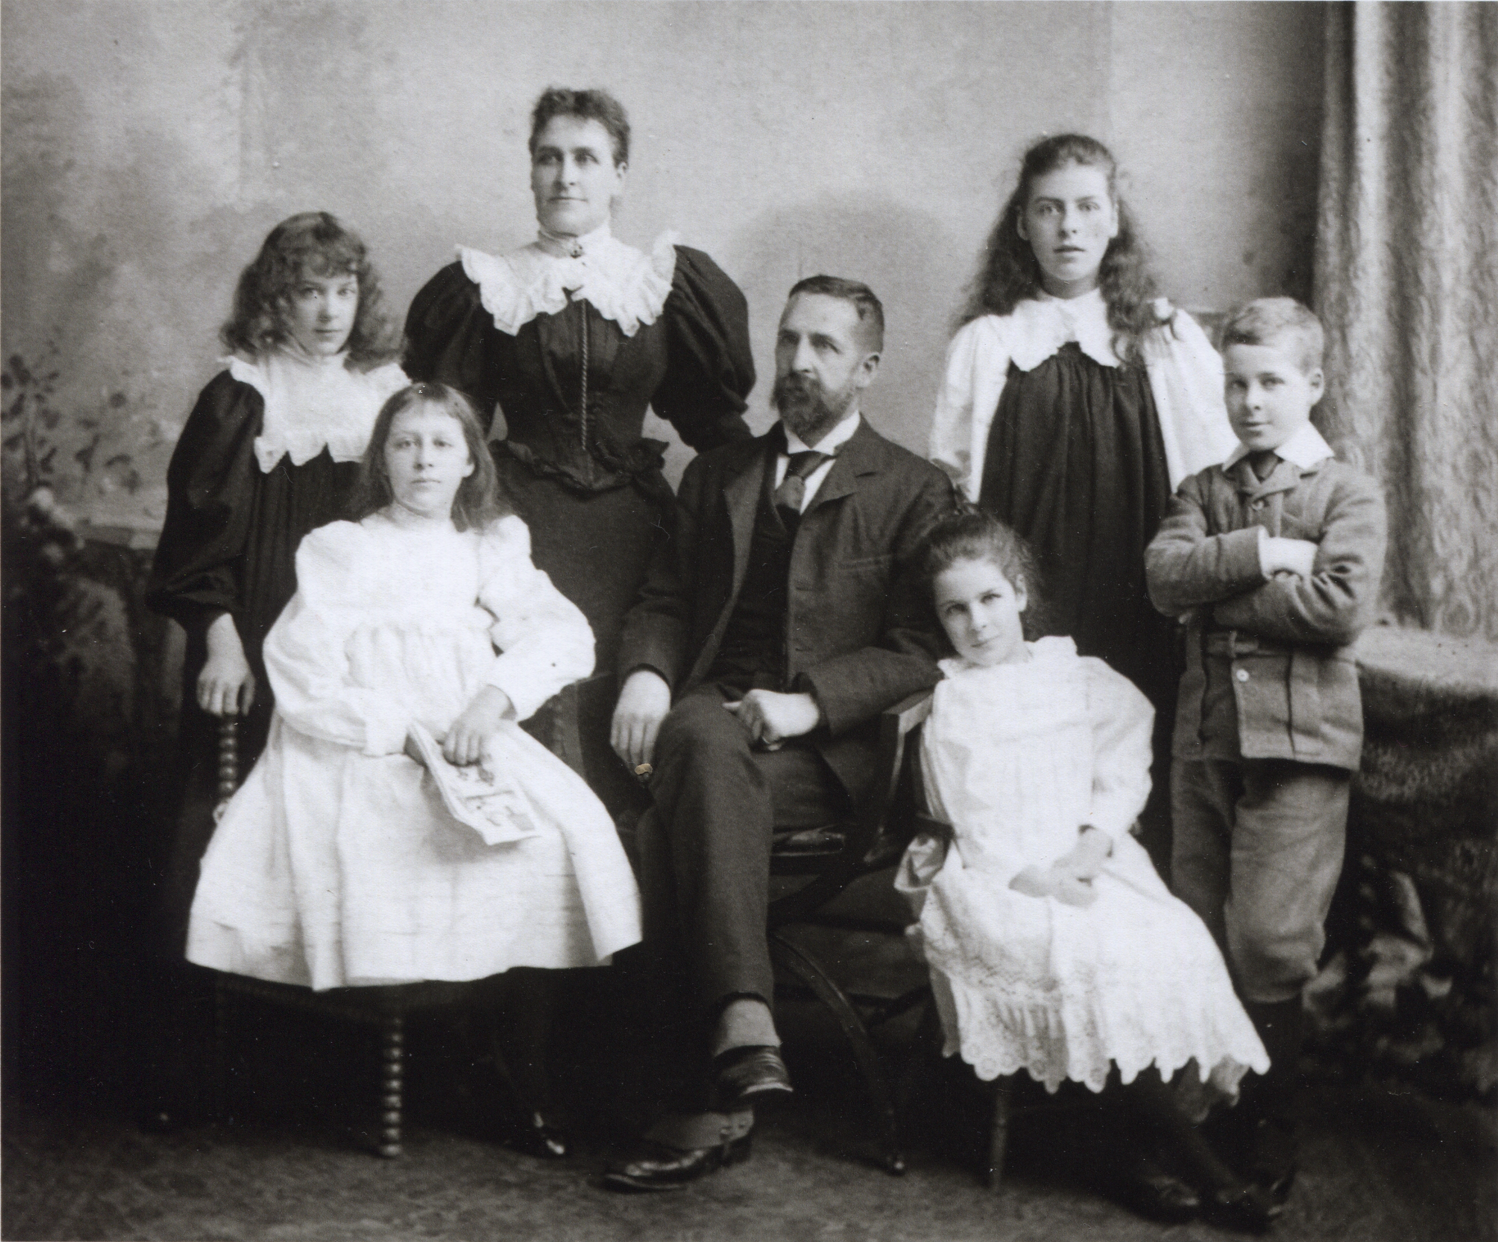
\includegraphics{photos/Munday_family}
	\caption{The Munday family c.~1900.\cite{MundayFamilyPhoto}}
\end{figure}

